\section{Stability Analysis}
%%%%%%%%%%%%%%%%%%%%%%%%%%%%%%%%
%%%%%%%%%%%%%%%%%%%%%%%%%%%%%%%%
% wx=pi
%%%%%%%%%%%%%%%%%%%%%%%%%%%%%%%%
%%%%%%%%%%%%%%%%%%%%%%%%%%%%%%%%

\begin{frame}{Stability analysis: Eigenvalues for large $D_r$}
	\scriptsize
	Example
	\begin{align*}
		\nabla_{x} \boldsymbol{u}_{\mathrm{ext}}=\left(\begin{array}{ccc}
			0 & 0 & 0 \\
			0 & 0 & 0 \\
			\pi & 0 & 0
		\end{array}\right)
	\end{align*}

\begin{figure}
	\begin{subfigure}{0.48\textwidth}
		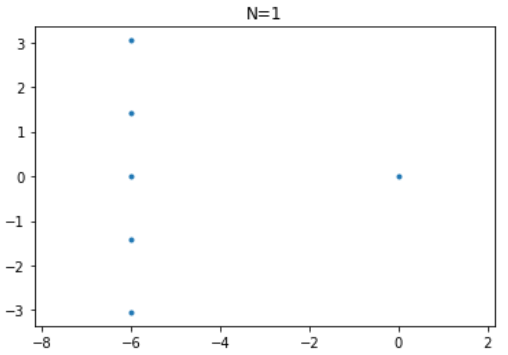
\includegraphics[width=\linewidth]{Bilder_wx/Stability/Ew_2nd_dr=1_dt=1}
	\end{subfigure}
	\hfill
	\begin{subfigure}{0.48\textwidth}
		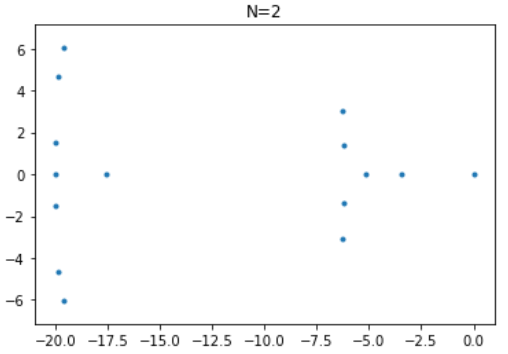
\includegraphics[width=\linewidth]{Bilder_wx/Stability/Ew_4th_dr=1_dt=1}
	\end{subfigure}
	\caption{Eigenvalues of matrix $A$ for $D_r = 1$}
\end{figure}
\end{frame}

\begin{frame}
	\begin{figure}
		\begin{subfigure}{0.48\textwidth}
			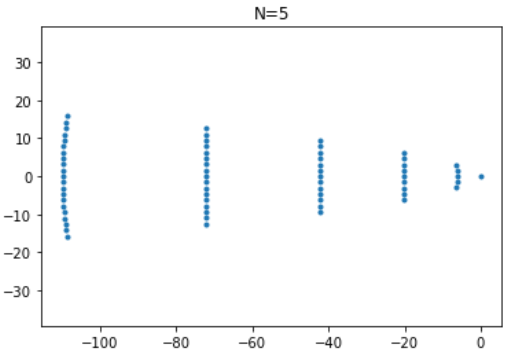
\includegraphics[width=\linewidth]{Bilder_wx/Stability/Ew_10th_dr=1_dt=1}
		\end{subfigure}
		\hfill
		\begin{subfigure}{0.48\textwidth}
			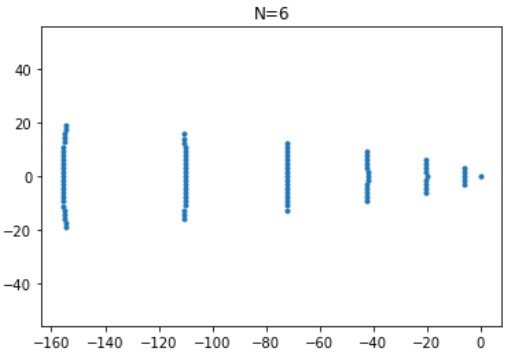
\includegraphics[width=\linewidth]{Bilder_wx/Stability/Ew_12th_dr=1_dt=1}
		\end{subfigure}
		\caption{Eigenvalues of matrix $A$ for $D_r = 1$}
	\end{figure}
	\begin{block}{Finding}
		An increase of the number of basis functions improves the stability of the spectral method
	\end{block}
\end{frame}

\begin{frame}{Absolute stability: for large $D_r$}
	\begin{figure}
		\begin{subfigure}{0.48\textwidth}
			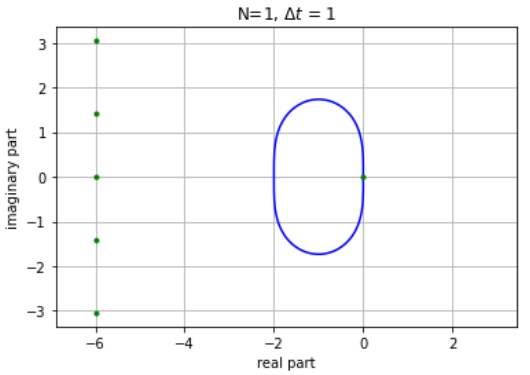
\includegraphics[width=\linewidth]{Bilder_wx/Stability/RK2_region_2nd_dr=1_dt=1}
		\end{subfigure}
		\hfill
		\begin{subfigure}{0.48\textwidth}
			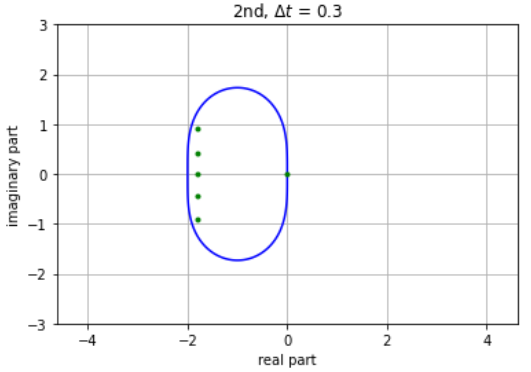
\includegraphics[width=\linewidth]{Bilder_wx/Stability/RK2_region_2nd_dr=1_dt=0.3}
		\end{subfigure}
		\caption{Stability region of $RK2$ with eigenvalues for $N=1$, $D_r=1$ and different time steps}
	\end{figure}
\end{frame}

\begin{frame}{Absolute stability: for large $D_r$}
	\begin{figure}
		\begin{subfigure}{0.48\textwidth}
			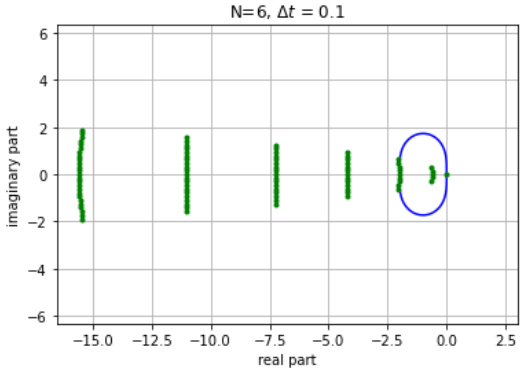
\includegraphics[width=\linewidth]{Bilder_wx/Stability/RK2_region_12th_dr=1_dt=0.1}
		\end{subfigure}
		\hfill
		\begin{subfigure}{0.48\textwidth}
			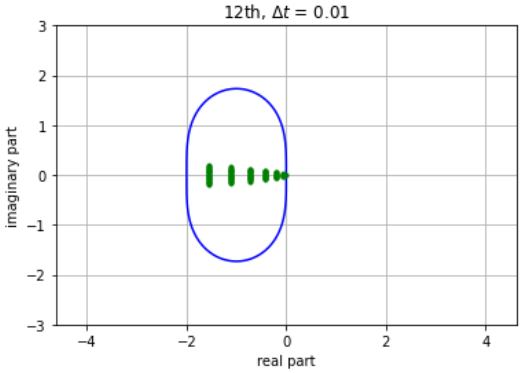
\includegraphics[width=\linewidth]{Bilder_wx/Stability/RK2_region_12th_dr=1_dt=0.01}
		\end{subfigure}
		\caption{Stability region of $RK2$ with eigenvalues for $N=6$, $D_r=1$ and different time steps}
	\end{figure}
	
	\begin{block}{Finding}
		For absolute stability for large $D_r$  $\rightarrow$ smaller time steps are needed
	\end{block}
\end{frame}